\chapter{Introducción}
\label{cap:capitulo1}
\setcounter{page}{1}

\begin{flushright}
\begin{minipage}[]{10cm}
\emph{El éxito es la suma de pequeños esfuerzos repetidos día tras día.}\\
\end{minipage}\\

Robert Collier\\
%Autor, \textit{Título}\\
\end{flushright}

\vspace{1cm}



%[Sección sobre la robótica y la importancia de la exploración espacial]
\section{La evolución y el estado de la robótica}
\label{sec:robotica} % etiqueta para luego referenciar esta sección

%[Párrafo sobre la definicion de robótica y de robot]
La robótica es un campo multidisciplinario que se concentra en el diseño,
construcción, programación y operación de robots.
Estos dispositivos electromecánicos, con frecuencia modelados
antropomórficamente o zoomórficamente, están destinados a realizar tareas de
manera autónoma o semiautónoma en una variedad de entornos, para lo que disponen
de sensores que les proveen de información del medio que les rodea, de cierta
capacidad de cómputo para tomar decisiones acerca de estos datos recolectados y
de actuadores que les permiten interactuar con el mismo y llevar a cabo dichas
decisiones, por lo que sus capacidades y limitaciones están detrminadas por su
\textit{hardware}, y su inteligencia reside en su \textit{software}.

%[Párrafo sobre la evolución de la robótica y su aplicación en nuestra sociedad]
Este gran campo de estudio e investigación ha experimentado un rápido
crecimiento y expansión desde sus inicios en la década de 1950, abarcando una
amplia gama de aplicaciones en la industria, la medicina, el entretenimiento y
la exploración espacial, entre muchas otras, y se encuentra en constante
evolución, desempeñando un papel cada vez más importante en nuestra sociedad
moderna, gracias en gran medida a los incesantes avances en tecnologías como la
inteligencia artificial, los sensores, los procesadores y los actuadores.



%[Sección sobre la importancia de la robótica en los avances científicos]
\section{La importancia de la robótica en la ciencia}
\label{sec:exploracion_espacial} % etiqueta para luego referenciar esta sección

%[Párrafo sobre la importancia de la propia exploración espacial]
En particular, la robótica ha conformado un factor crucial en la exploración
espacial, y esta ha impulsado la creación de nuevas tecnologías que han sido
desarrolladas exclusivamente para ciertas misiones espaciales pero que luego se
han aplicado en la Tierra, mejorando la calidad de vida de las personas.
Ejemplos destacados incluyen los sistemas de purificación de agua, los tejidos
avanzados como la viscoelástica, los pañales y los dispositivos de imágenes
médicas como la resonancia magnética, que han proporcionado acceso a las
personas respectivamente a agua potable en regiones remotas, a colchones y
almohadas que promueven un mejor descanso, a mayores facilidades en cuanto al
cuidado de los niños y mayores y a diagnósticos médicos precisos sin radiación
nociva, lo cual ha salvado inumerables vidas.
De esta manera, la investigación espacial no solo expande nuestro conocimiento
del universo, sino que también beneficia directamente a la humanidad en la
Tierra.

%[Párrafo sobre el rover Perseverance y el helicóptero Ingenuity]
En cuanto al papel de la robótica en este campo, podemos destacar ejemplos como
los resistentes robots enviados a diferentes planetas y lunas del sistema solar
en busca de datos científicos.
Numerosas misiones científicas lo evidencian, como la misión \textit{Mars 2020}
de la NASA, cuyos robots se ven ilustrados en la Figura \ref{fig:rover}, tomada
por uno de los robots, el rover Perseverance, que depositó con éxito al segundo
robot sobre la superficie marciana, el helicóptero Ingenuity, que aparece más al
fondo en la imagen, y que ayudó al rover a llevar a cabo su exploración y toma
de muestras.
Este helicóptero estaba diseñado para realizar 5 vuelos durante un mes a modo de
demostrador tecnológico, pero su misión pudo alargarse hasta casi los 3 años,
momento en el que termina debido a la rotura de una de sus palas, sumando
entonces un total de 72 vuelos.

\begin{figure} [h!]
  \begin{center}
    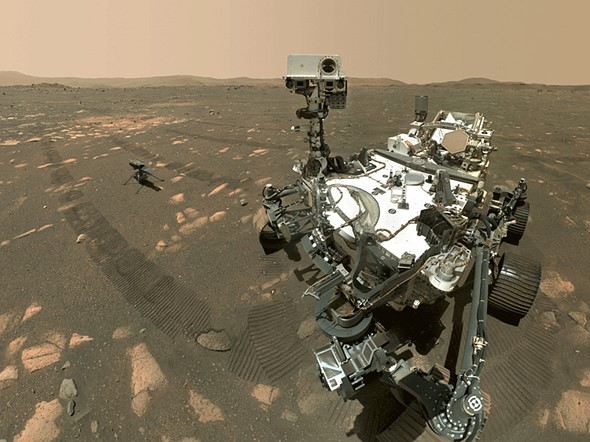
\includegraphics[width=8cm]{figs/perseverance_and_ingenuity_mars_rover_selfie}
  \end{center}
  \caption{Rover Perseverance y helicóptero Ingenuity de la NASA en Marte.}
  \label{fig:rover}
\end{figure}\

%[Párrafo de enlace con la robótica móvil]
Para el éxito de esta misión fue clave la investigación en múltiples campos de
la robótica, como la robótica móvil y todos los campos que esta conlleva, como
pueden ser la visión artificial, la navegación o la localización, áreas clave
que no solo están redefiniendo los límites de la tecnología, sino que también
tienen un gran impacto en cómo usamos la tecnología en nuestra vida diaria, como
ha sucedido por ejemplo, con las aspiradoras robóticas o la conducción
autonoma, que inevitablemente ya forman parte de nuestra sociedad.



%[Sección sobre la robótica móvil y su relación con la educación]
\section{La robótica móvil en relación con la educación}
\label{sec:robotica_movil} % etiqueta para luego referenciar esta sección

%[Párrafo sobre la robótica móvil]
La robótica móvil ha emergido como un campo multidisciplinario que fusiona la
ingeniería, la inteligencia artificial y múltiples ramas de la robótica y la
mecatrónica para crear sistemas capaces de moverse y operar en entornos
dinámicos, aprovechando áreas como la robótica de campo, la creación de mapas,
la localización y la navegación con ayuda de otros como la visión artificial o
la manipulación de objetos.

Desde sus inicios, ha sido impulsada por los avances tecnológicos, permitiendo
su aplicación en una amplia gama de campos, desde la exploración espacial y
submarina, hasta la logística industrial y la atención médica, siendo ya parte
indispensable de nuestras vidas y mejorando la calidad de las mismas.
En este contexto, la investigación en robótica móvil se centra en desarrollar
sistemas autónomos capaces de navegar de manera segura y eficiente en entornos
conocidos o desconocidos, adaptarse a cambios imprevistos y realizar tareas
complejas de manera autónoma.

Un ejemplo representativo de este tipo de robots se puede ver en la Figura
\ref{fig:boston_dynamics}, donde se pueden observar dos de los robots más
desarrollados en el ámbito móvil, que han demostrado una gran versatilidad en
una variedad de entornos para ejecutar una amplia variedad de tareas, desde
abrir puertas, pasando por transportar cargas de peso o realizar trabajos
manuales, hasta incluso seguir rutinas de deportivas variadas, que en muchos
casos iguala o incluso supera la de los humanos.

\begin{figure} [h!]
  \begin{center}
    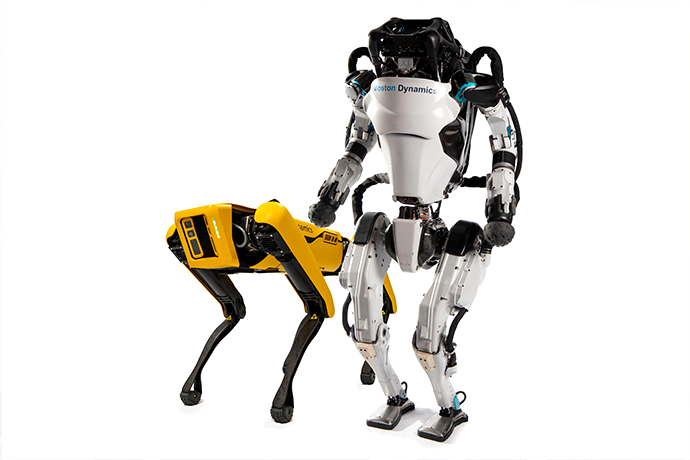
\includegraphics[width=8cm]{figs/atlas_spot_boston_dynamics}
  \end{center}
  \caption{Robots Spot (izq.) y Atlas (dcha.) de Boston Dynamics.}
  \label{fig:boston_dynamics}
\end{figure}\

%[Párrafo introductorio a la localización]
En concreto, la localización de los robots juega una papel importante en la
robótica móvil debido a su indispensable necesidad a la hora de navegar por el
entorno normalmente tomando puntos de referencia gracias a los sensores y
creando un modelo probabilístico de la posición del robot basado en estos datos.

%[Párrafo introductorio a la navegación]
Por su parte, para el correcto funcionamiento de la navegación, es indispensable
conocer la posición del robot durante el movimiento del mismo, para tener la
capacidad de sortear obstáculos y poder desplazar el robot al objetivo.

%\cite{Trawny2009} %multilocalización probabilistica cooperativa unidimensional,
%                  %filtro kalman.
%\cite{Fox2000}    %multilocalización probabilistica basada en sensores y
%                  %balizas visuales.
%[Párrafo introductorio a la multirobótica y trabajos de localización]
La robótica móvil también forma parte de campos más grandes y complejos e
incluso sienta las bases de algunos de ellos, como sucede con la multirobótica,
que representa un paso adelante en la complejidad y la escala de los sistemas
robóticos individuales, y permite realizar tareas que un solo robot no es capaz
de hacer, o realizarlas mucho mas rápidamente o eficientemente.
Como ejemplo de esta ventaja, son notables ciertos trabajos realizados sobre
localización con múltiples robots, como en el artículo \cite{Trawny2009}, en el
que se ponen a prueba las mismas técnicas utilizadas para un solo robot y
evalúan su viabilidad en un entorno unidimensional.
También se han realizado trabajos enfocados a entornos tridimensionales, como se
observa en el artíulo \cite{Fox2000}, en el cuál se logra una localización
basada en sensores, teniendo en cuenta la posición de los demás robots y
aumentando de este modo la precisión de la localización del propio robot en
cuestión.

%[Párrafo sobre la educación en relación con la robótica móvil]
Además, este campo supone una gran oportunidad para el aprendizaje, ya que juega
un papel crucial en el desarrollo de habilidades tecnológicas a la vez que en la
motivación de los estudiantes, los cuales obtienen una gran sensación de
realización y entusiasmo por aprender, al poder viualizar los resultados en
movimiento de manera autonoma.



%[Sección sobre la educación en robótica]
\section{La educación en robótica}
\label{sec:educacion_robotica} % etiqueta para luego referenciar esta sección

%[Párrafo sobre la demanda de educación en robótica en el mundo]
Debido a la creciente participación de los robots móviles en nuestras vidas
diarias, como se ha hecho notar en el caso de las aspiradoras robóticas, la
relevancia de la robótica en el ámbito educativo ha ido ganando terreno en los
últimos años, tanto en la comunidad europea como en otros muchos países.
Esto ha dado lugar a un aumento en la implementación de programas educativos que
han incluido actividades prácticas de robótica en escuelas de educación primaria
y secundaria, promoviendo la creatividad, el pensamiento crítico y las
habilidades tecnológicas entre los estudiantes, además de fomentar el trabajo en
equipo y la resolución de problemas complejos, preparándolos para futuros grados
o carreras relacionadas con la tecnología, cuya demandada aumenta
incesablemente.

%[Párrafo sobre la educación en robótica en España]
En el caso de España, desde la década de los 90, se han implementado programas
piloto y competiciones robóticas, como el programa
Robolot\footnote{\url{https://www.robolot.online/}} (1992), desarrollado por la
UPC, las Olimpiadas de
Informática\footnote{\url{https://olimpiada-informatica.org/}} (1993), que
incorporaron desafíos relacionados con la programación de robots, así como la
RoboCupJunior\footnote{\url{https://junior.robocup.org/}} (2000), ofreciendo a
los estudiantes la oportunidad de diseñar, construir y programar robots para
competir en diferentes categorías.
Desde alrededor de 2014, dependiendo de la comunidad autónoma de España, se han
introducido programas y asignaturas que incluyen la robótica como parte esencial
del plan de estudios.

%[Párrafo sobre las herramientas utilizadas en la educación en róbotica]
Al ser necesario un contexto simple y barato para la introducción a la robótica,
en la educación se buscan herramientas como las placas Arduino (Figura
\ref{fig:arduino}), que presentan una amplia compatibilidad con distintos
sensores y actuadores y brinda un entorno sencillo para aquellos que se están
introduciendo en este campo y plataformas como
\textit{Scratch}\footnote{\url{https://scratch.mit.edu/}} para simplificar la
programación gracias a su interfaz de bloques y la asociación de ideas a
colores, como se muestra en la Figura \ref{fig:scratch}.

\begin{figure}[h!]
  \centering
  \begin{minipage}{0.45\textwidth}
    \centering
    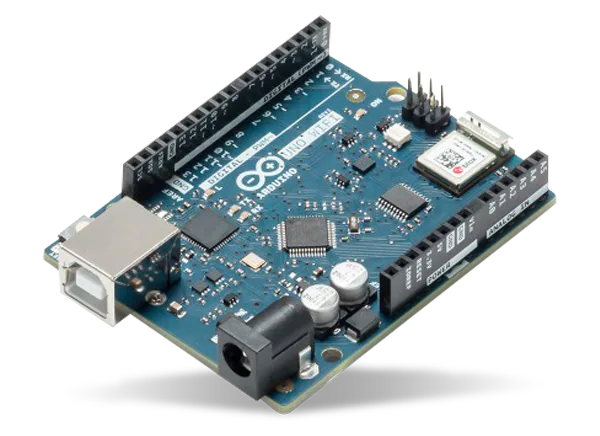
\includegraphics[width=7cm]{figs/arduino}
    \caption{Arduino.}
    \label{fig:arduino}
  \end{minipage}
  \hfill
  \begin{minipage}{0.45\textwidth}
    \centering
    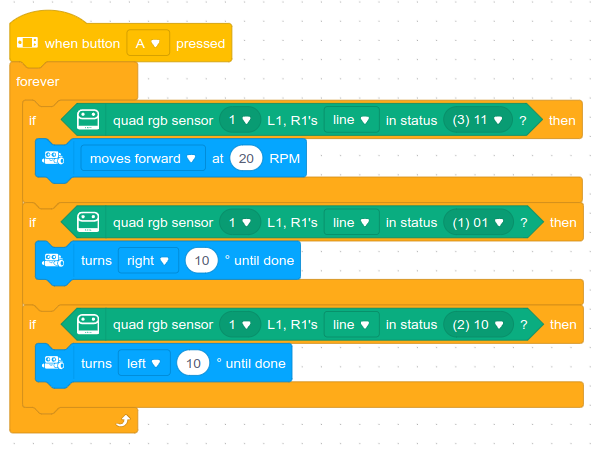
\includegraphics[width=7cm]{figs/scratch_arduino_code}
    \caption{Código de Arduino en Scratch.}
    \label{fig:scratch}
  \end{minipage}
\end{figure}\

%[Párrafo sobre la educación en relacion con la robótica móvil]
Las placas utilizadas en el ámbito educativo, mencionadas anteriormente,
resultan ideales para estos propósitos debido a su coste y simplicidad, sin
embargo, también imponen ciertas limitaciones en las capacidades del robot y en
la posibilidad de añadir \textit{hardware} externo más complejo y potente, como
cámaras o LIDARs, o actuadores como motores más potentes que a menudo requieren
de mayor alimentación eléctrica de la que estas placas pueden brindar.
Esto genera trabas a la propia originalidad y aprendizaje de los estudiantes,
restringiendo así su creatividad, innovación y potencial de creación, una vez se
han obtenido unos conocimientos básicos.

%[Párrafo sobre el escalón de aprendizaje en la educación en robótica]
Es entonces cuando se encuentra el desafío de dar el siguiente paso: la
programación de robots utilizando ROS, el \textit{middleware} estándar por
excelencia en robótica.
Este proceso implica un considerable escalón de aprendizaje, ya que no solo se
debe dominar un lenguaje de programación más complejo, sino que también se debe
comprender el entorno que rodea a esta plataforma, en el que se incluyen campos
de la robótica como son las comunicaciones, la arquitectura \textit{software},
la programación modular y orientada a objetos, algoritmos y estructuras de
datos, entre otros muchos, y que suelen conllevar decenas de asignaturas con
identidad propia en cualquier grado de universidad.
La teoría de la existencia de una brecha educativa en este ámbito se ve
respaldada por trabajos como la tesis doctoral de \cite{vega18b}, en cuyas
secciones A.3 y A.4, se analiza esta misma perspectiva y se propone una solución
respectivamente.

Dicha complejidad puede verse ilustrada en la Figura \ref{fig:ros}, en la que se
muestra un esquema simplificado de la arquitectura de ambas versiones de este
\textit{middleware} que puede resultar abrumadora para aquellos que se están
iniciando en este ámbito, ya que se muestra la creciente complejidad adquirida
al pasar de ROS, que ya era suficientemente complejo, a ROS2, en el que ahora
existen distintas implementaciones de \textit{middleware} de comunicaciones, y
otras capas como al de transporte, el sistema operativo y el \textit{hardware}.

\begin{figure} [h!]
  \begin{center}
    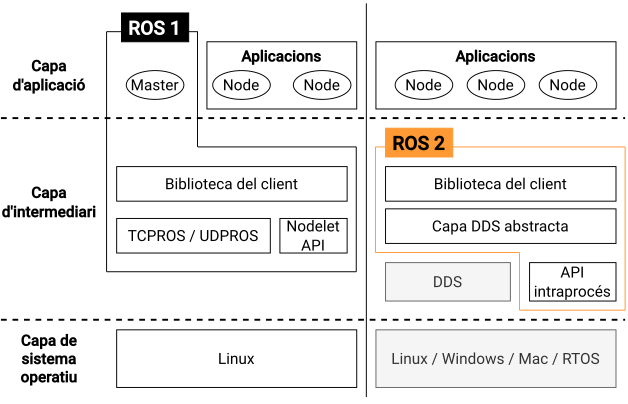
\includegraphics[width=12cm]{figs/ROS_and_ROS2}
  \end{center}
  \caption{Arquitectura de ROS y ROS2.}
  \label{fig:ros}
\end{figure}\

%[Párrafo sobre la solución al escalón de aprendizaje en robótica]
Por este motivo, resulta evidente la necesidad de un paso intermedio que pueda
actuar como puente entre estos dos niveles de aprendizaje, el cual podría ser
incorporado, por ejemplo, en el programa educativo del bachillerato tecnológico
o de centros de educación secundaria.
Este nivel intermedio facilitaría la transición entre las habilidades adquiridas
en la enseñanza primaria o secundaria y los requisitos más avanzados de la
universidad en el campo de la robótica.



%[Sección sobre la robótica de bajo coste]
\section{La robótica de bajo coste}
\label{sec:robotica_bajo_coste} % etiqueta para luego referenciar esta sección

%[Párrafo sobre la robótica de bajo coste]
La robótica de bajo coste se refiere al desarrollo e implementación de sistemas
robóticos como los descritos anteriormente utilizando componentes y recursos
económicos, con el objetivo de hacer la tecnología robótica más accesible y
asequible para una amplia gama de aplicaciones y usuarios.
Este enfoque busca reducir los costes asociados con la construcción y operación
de robots, empleando materiales económicos, hardware de bajo coste y técnicas
de fabricación eficientes.

%[Párrafo sobre la robótica de bajo coste en relación con la robótica móvil]
En el contexto de la robótica móvil, los sistemas de bajo coste pueden ofrecer
soluciones viables para aplicaciones con presupuestos limitados o despliegues a
gran escala, abarcando un papel crucial en áreas como la educación, la
investigación académica, la asistencia social y la exploración de entornos
remotos o peligrosos.
Además de su utilidad práctica, la robótica de bajo coste también promueve la
innovación y el desarrollo de nuevas tecnologías al proporcionar una plataforma
accesible para la experimentación y la creatividad abierta a una amplia
comunidad, así como a la educación.

%[Párrafo ejemplificativo sobre la robótica de bajo coste]
Un ejemplo destacado de este tipo de robótica es el robot Sora-Q representado en
la Figura \ref{fig:sora_q}, enviado a la Luna recientemente por la JAXA y
desarrollado por una empresa de juguetería japonesa, y que tras completar su
misión, fue comercializado por 150\euro, hito que ilustra cómo la tecnología
robótica puede volverse accesible para un público más amplio, incluso
después de su participación en misiones espaciales.

\begin{figure} [h!]
  \begin{center}
    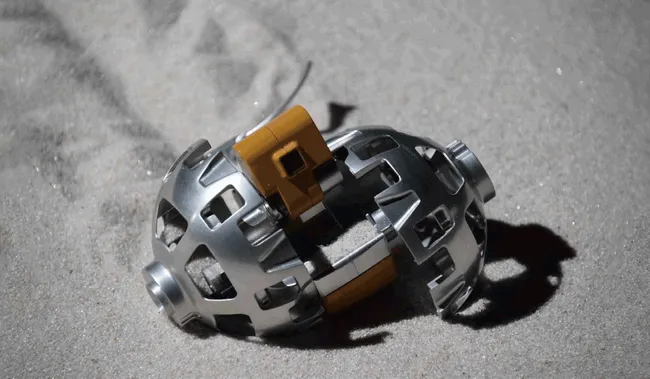
\includegraphics[width=8cm]{figs/SoraQ_lunar_robot_JAXA}
  \end{center}
  \caption{Sora-Q, robot lunar \textit{low-cost} desarrollado por Takara Tomy y la JAXA.}
  \label{fig:sora_q}
\end{figure}\

%[Párrafo sobre la robótica de bajo coste en relación con la educación]
La educación en robótica suele basarse en este tipo de sistemas de bajo coste,
ya que las instituciones educativas enfrentan limitaciones presupuestarias que
dificultan la adquisición de sistemas más costosos, por su gran número de
alumnos, a los que no podrían proveer de sistemas de este calibre de otra
manera.

%[Párrafo sobre los beneficios de la robótica de bajo coste en la educación]
La robótica de bajo coste no solo ha democratizado el acceso a la tecnología
robótica, sino que también ha revolucionado la forma en que se enseña la
robótica en las escuelas.
Este enfoque económico ha permitido a las instituciones educativas superar las
limitaciones presupuestarias y proporcionar a un mayor número de estudiantes la
oportunidad de involucrarse en actividades prácticas de robótica, allanando el
camino para que los estudiantes se sumerjan en áreas más avanzadas de este área,
como pueden ser la robótica móvil o campos estrechamente relacionados.



%[Sección sobre la multirobótica]
\section{La multirobótica}
\label{sec:multirobotica} % etiqueta para luego referenciar esta sección

%\cite{Verma2021}      %Resumen de multirobotica en general.
%\cite{Parker2003}     %Subcampos de multirobotica explicados (comunicación, la
%                      %planificación de tareas, la localización, la creación de
%                      %mapas, la manipulación de objetos, la coordinación de
%                      %robots, o robótica reconfigurable...).
%\cite{Sheng2006}      %Enfocado a descentralizacion, coordinacion y
%                      %optimizacion.
%\cite{Alami1998}      %Cooperacion, menor centralizacion, programar cada robot.
%\cite{Chaimowicz2001} %Coordinacion centralizada, los robots tienen la
%                      %capacidad de cambiar de rol.

%[Párrafo introductorio sobre la multirobótica]
La multirobótica es un campo de investigación que estudia y desarrolla sistemas
robóticos compuestos por múltiples robots que trabajan en conjunto para realizar
una variedad tareas complejas, que ha sido ampliamente estudiada en artículos
como \cite{Verma2021}, en los que se relatan todos los aspectos de la misma,
poniendo en contexto este novedoso campo.

%[Párrafo más específico sobre las tareas más relevantes en la multirobótica]
Estos sistemas pueden dividir sus tareas, como la exploración de entornos
desconocidos o la búsqueda y rescate en áreas de difícil acceso, por lo que la
colaboración entre ellos es de vital importancia, e implica aspectos como el
establecimiento de comunicaciones para compartirse información y entender de un
mejor modo el mundo y contexto que les rodea, la creación de mapas del entorno
para poder localizarse y navegar por el mismo de manera controlada o la
manipulación de objetos, muchas veces necesaria para completar el objetivo
propuesto para estos sistemas.
Todo ello puede verse descrito en al trabajo de \cite{Parker2003}, en el que se
relatan con más detalle los avances logrados en estos aspectos.

%[Párrafo sobre la importancia de la coordinación en la multirobótica]
La coordinación entre estos sistemas puede suponer la diferencia entre el éxito
o el fracaso de su misión, por lo que también es de suma importancia, y por ello
se han realizado múltiples trabajos acerca de este tema.
En estos términos, los equipos de robots pueden operar eficientemente
asignando roles y responsabilidades como expone el artículo de \cite{Alami1998},
en el que se desarrolla un sistema de control con la menor centralización
posible para estudiar la cooperación multirobot en el proyecto
MARTHA\footnote{MARTHA: European ESPRIT III Project No 6668 \textquotedblleft
Multiple Autonomous Robots for Transport and Handling
Applications\textquotedblright}.

%[Párrafo sobre la descentralización en la multirobótica]
A pesar de intentar crear sistemas con la mayor descentralización posible, el
trabajo anterior sigue siendo un sistema centralizado, donde un robot puede
asumir roles específicos.
La tendencia actual se inclina hacia sistemas directamente o casi totalmente
descentralizados, donde la coordinación y la optimización son fundamentales,
como es notable en el trabajo de \cite{Sheng2006}, en el que todos los robots
actualizan su propio mapa local con la información de los demás, sin que ninguno
de ellos adquiera un mayor protagonismo o importancia.

Gracias a este tipo de trabajos, se ha conseguido mejorar la eficiencia y la
robustez de los sistemas robóticos, y la multirobótica se ha convertido en un
campo importante de investigación.
Los principios y problemas técnicos en este campo se exploran en diversos
contextos, como se ilustra en la Figura \ref{fig:multirobots}, en la cual, la
flota de robots está realizando una tarea de búsqueda y rescate, mediante la
división de un área, probablemente desconocida, actualizando sus mapas como
se ha explicado anteriormente.

\begin{figure} [h!]
  \begin{center}
    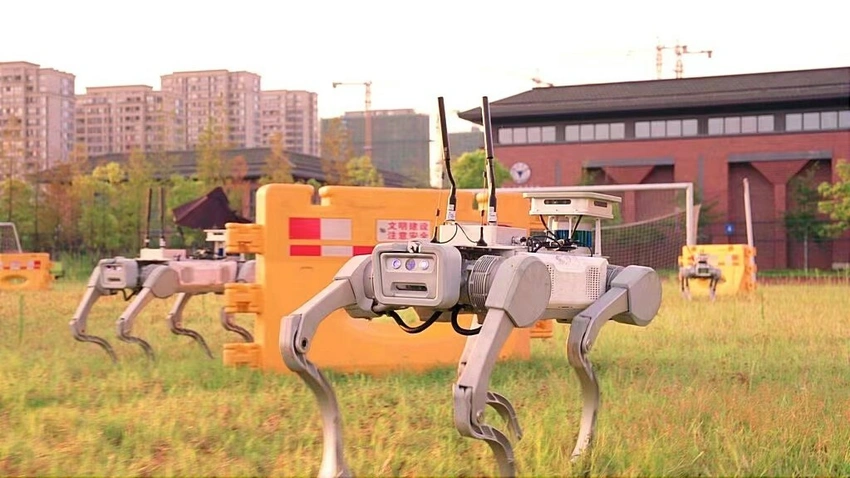
\includegraphics[width=8cm]{figs/multirobotics_in_search_and_rescue}
  \end{center}
  \caption{Múltiples robots durante una operacion de búsqueda y rescate.}
  \label{fig:multirobots}
\end{figure}\

%[Párrafo sobre la multirobótica en educación].
En el ámbito educativo, la multirobótica ofrece una oportunidad única para
involucrar a los estudiantes en actividades prácticas y colaborativas.
Al trabajar con sistemas multirobot, los estudiantes no solo adquieren
conocimientos sobre programación, control y mecánica de robots, sino que también
exploran conceptos como son las telecomunicaciones entre robots, la coordinación,
la planificación y asignación de tareas con o sin prioridades, la localización y
navegación conjunta, como se ha explicado en los trabajos citados en la sección
\ref{sec:robotica_movil}, así como la seguridad que se requiere para evitar
colisiones entre ellos, adquiriendo a su vez habilidades útiles para el trabajo
en equipo.
Además, la multirobótica proporciona un entorno de aprendizaje dinámico y
estimulante que despierta aún más la curiosidad y la creatividad de los
estudiantes, preparándolos para enfrentar los desafíos del mundo tecnológico en
constante evolución.

%[Párrafo sobre ejemplos de múltiples robots educativos].
Un ejemplo representativo de los robots educativos, en este caso del laboratorio
de robótica de la URJC, aparece en la Figura \ref{fig:robots_education}, en la
que se pueden diferenciar hasta dos modelos distintos de robots: Turtlebot 2 en
la parte superior de la imagen, y Turtlebot 4, más modernos, en la parte inferior
de la misma.

\begin{figure} [h!]
  \begin{center}
    \includegraphics[width=8cm]{figs/multirobotics_education}
  \end{center}
  \caption{Robots educativos, modelos Turtlebot 2 (arriba) y Turtlebot 4 (abajo).}
  \label{fig:robots_education}
\end{figure}\



%[Sección sobre los flujos de datos en robótica]
\section{Flujos de datos en robótica}
\label{sec:flujos_datos} % etiqueta para luego referenciar esta sección

%[Párrafo sobre las telecomunicaciones entre robots]
Las mencionadas telecomunicaciones entre robots son fundamentales en la
multirobótica, ya que garantizan una comunicación rápida, optima, eficiente y
ordenada entre los distintos dispositivos, necesaria para un correcto desempeño
de la funcionalidad en cuestión.
Sin embargo, este proceso puede enfrentarse a desafíos como la congestión de la
red, y la consecuente pérdida de mensajes, que pueden ser críticos para el
correcto funcionamiento de los robots.
Por este motivo es crucial gestionar cuidadosamente la cantidad de robots y
mensajes generados, intentando minimizarlos para optimizar el rendimiento del
sistema y evitando de esta manera el problema conocido como \textquotedblleft
cuello de botella\textquotedblright.

%[Párrafo sobre ZettaScale]
Una de las empresas más importantes en este ámbito es ZettaScale Technology, que
ha tomado mucha relevancia en los últimos años, ya que es responsable de una de
las implementaciones de \textit{middleware} de telecomunicaciones de DDS
utilizado en ROS2, llamado \textit{CycloneDDS} y son los desarrolladores de un
reciente protocolo de comunicaciones llamado \textit{Zenoh}, que ya cuenta con
importantes clientes como la NASA, debido a las prestaciones que este ofrece,
superando en la mayoria de casos a los protocolos convecionales y que ya ha sido
oficialmente seleccionado como el próximo RMW de
ROS2\footnote{\url{https://discourse.ros.org/t/ros-2-alternative-middleware-report/33771}}.
Además de esto poseen un potente middleware para la programación de flujos de
datos aún en desarrollo, llamado \textit{Zenoh-Flow}, así como un puente llamado
\textit{zenoh-bridge-dds} que hace las veces de traductor entre los protocolos
DDS y Zenoh, lo que permite la comunicación entre estos flujos de datos con
nodos de ROS2, haciendo posible la creación de aplicaciones robóticas en forma
de flujos de datos, utilizando nodos de ROS2 existentes, y fusionando de esta
manera ambos campos.

%[Párrafo sobre flujos de datos y comportamiento reactivo mas simple para educación]
Un flujo de datos consiste en un grafo dirigido de los datos que fluyen entre
operaciones.
Mantener un flujo de datos correcto es fundamental para solventar los problemas
de telecomunicaciones mencionados en el desarrollo de sistemas de multirobótica.
Además, simplifica el desarrollo del software al proporcionar una clara visión
de la dirección, el origen y el destino de los datos en cada momento.
Esto permite dividir el programa en partes claramente diferenciadas, normalmente
llamadas nodos, modularizándolo y dando lugar a la división del problema último
en varios problemas más simples y fáciles de atajar, creando un paradijma que
modela el programa como un flujo de datos.
Como resultado, el desarrollo se vuelve un proceso más sostenible y escalable, y
por tanto, más fácil de llevar a cabo por los estudiantes.

Este proceso se puede ver representado en la Figura
\ref{fig:data_flow_qr_example}, donde se ilustra el flujo de datos de manera
simplificada, de un robot para detectar y seguir códigos
QR\footnote{\url{https://github.com/USanz/follow_beacon}}, en la que se puede
observar cómo los datos siguen un esquema de nodos dirigido, y en este caso
unidireccional, pasando de su orígen en el robot a su procesamiento en otra
máquina y acabando en su posterior vuelta al robot en forma de ordenes de
movimiento, pudiendo saber en todo momento en qué proceso se encuentran dichos
datos.

\begin{figure} [h!]
  \begin{center}
    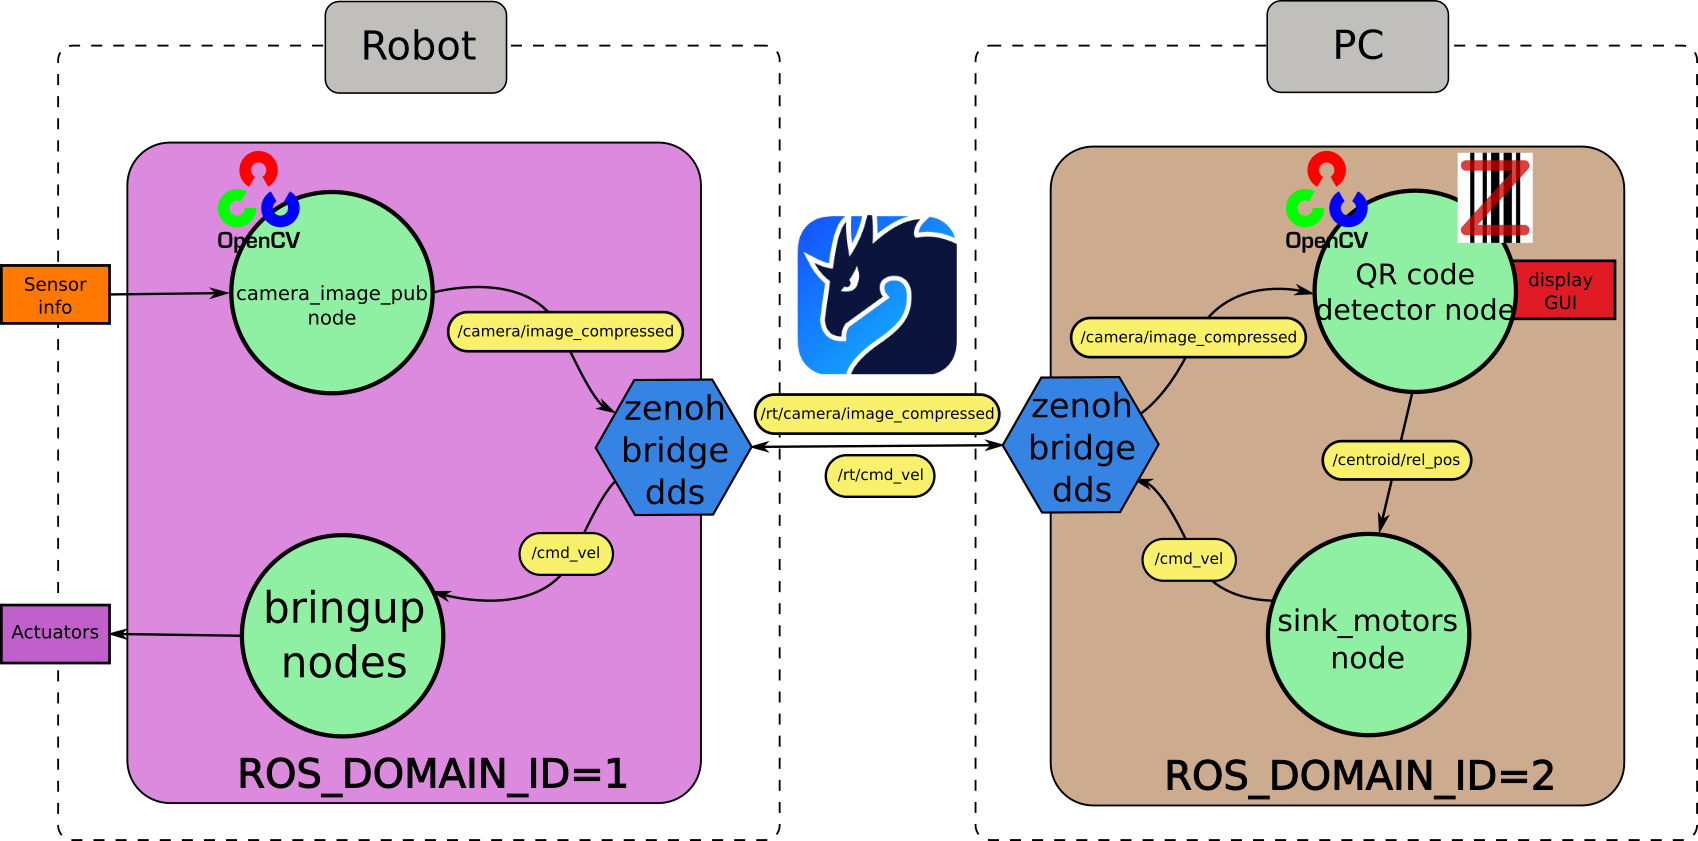
\includegraphics[width=15cm]{figs/QR_code_data_flow}
  \end{center}
  \caption{Flujo de datos de un robot para la detección y seguimiento de códigos QR.}
  \label{fig:data_flow_qr_example}
\end{figure}\

Este proceso es equiparable a la forma de programacióm de un robot reactivo, ya
que, como se observa en la figura \ref{fig:data_flow_vs_robotics}, en los flujos
de datos existen tres tipos esenciales de nodos: unos en los que se originan los
datos, otros donde se comutan y otros donde los datos llegan a su final; y que
encuentran correspondencia en los nodos encargados de la percepción de un robot,
del computo de estos datos obtenidos y de los nodos encargados de la actuación
del robot, respectivamente.
Todo ello se ve mejor explicado en una charla en la conferencia ROSCON Madrid de
2023\footnote{\url{https://www.youtube.com/watch?v=ZgFHCvEFU0I}}

\begin{figure} [h!]
  \begin{center}
    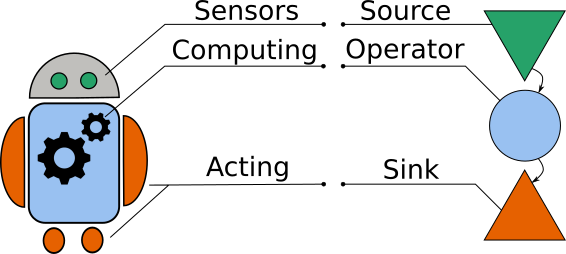
\includegraphics[width=9cm]{figs/data-flow_vs_robotics_scheme}
  \end{center}
  \caption{Comparación de un flujo de datos con los componentes de un robot.}
  \label{fig:data_flow_vs_robotics}
\end{figure}\

Además, este tipo de programación de los robots de manera reactiva es el más
simple y el primero que se suele aprender, por lo que genera una sinergia con la
educación en este ámbito.



%[TODO] Eliminar comentarios sobrantes al final (moverlos a su sección).
%[TODO] Capitulo II Estado del arte (no necesario si cito bien todo en la introduccion).
%[TODO] Hacer collage de las imagenes del video para explicar en varios pasos lo mismo que el video.
%[TODO] Poner las URLs como notas al pie. Ej: Robocup\footnote{\url{http://www.robocup.org}}.
%[TODO] Poner las URLs de videos en las notas al pie de página??

%[TODO] Capitulo II: objetivos y metodologia
%[TODO] buscar objetivos que se deben cumplir en los tfgs de la universidad y añadir los que se han cumplido











%[TODO] Párrafo de la antigua introducción que debería ser movido posiblemente
% al siguiente capitulo (hay cosas repetidas):

%La educación en robótica se basa en la robótica de bajo coste, normalmente en
%placas como Arduino o similares, las cuales son ideales para este uso, y a su
%vez limitan la capacidad del robot en cuestión y el hardware que se puede usar y
%consecuentemente limitan la creatividad y el aprendizaje de los niños. Una vez
%se llega a un cierto nivel de conocimientos, el siguiente paso suele ser la
%programación de robots con ROS2, donde existe un gran escalon de aprendizaje.
%Este trabajo busca simplificar el desarrollo del software en ROS2 y así reducir
%dicho escalón, para hacer más fácil este desarrollo, dando la posibilidad de
%crear aplicaciones robóticas más complejas para robots más completos y que
%permanecen dentro de la categoría de robots de bajo coste y por tanto siguen
%siendo asequibles para instituciones como colegios o institutos.\\

%Escribe aquí un párrafo explicando brevemente lo que vas a contar en este capítulo. En este primer capítulo, el de introducción, se trata de dar un contexto amplio y atractivo del trabajo. Comienza hablando de un contexto general y acaba hablando del contexto más específico en el que se enmarca el proyecto. Es el capítulo idóneo para incluir todas las referencias bibliográficas que hayan tratado este tema; suponen un fuerte respaldo al trabajo.\\

%\section{Problemas de ROS en relación con el aprendizaje}
%\label{sec:miseccion} % etiqueta para luego referenciar esta sección

%\section{Problemas de ROS en relación con el aprendizaje}
%\label{sec:miseccion} % etiqueta para luego referenciar esta sección

%ROS es el estándar en robótica para la programación de robots, pero tiene un
%problema y es el gran escalón de aprendizaje que existe cuando se pasa de una
%placa simple como arduino, a robots más complejos con máquinas integradas como
%las placas Raspberry Pi o un ordenador portátil directamente. Esto conlleva a una gran
%diferencia entre la robótica que se enseña en los colegios e institutos a la que
%se ebnseña en universidades, y es debido precisamente a la complejidad de código
%y enseñanza de ROS, para los cuales, se requiere incluso de varias asignaturas.
%Por eso en este trabajo se pretende incorporar un paso intermedio en este gran
%escalón.
%
%La propia naturaleza de este \textit{middleware} robótico nos obliga a programar
%nodos que se ejecutan iterativamente en bucle, sin necesidad de generar una
%topología de red concreta para saber de donde vienen o a donde van los datos, lo
%que puede ser un poco complicado de entender a primera vista para los niños.\\
%
%Además de este problema, existe otro relacionado con la congestión de red: los
%nodos de ROS2 se comunican a través de DDS, un protocolo de comunicaciones que
%genera una gran cantidad de mensajes de \textit{Discovery}, lo que conlleva
%consecuentemente a la generación de congestión de la red, y dificulta de esta
%manera la programacion de aplicaciones multirobóticas, que son un posible
%siguiente paso en la enseñanza de la robotica, para entender las comunicaciones
%entre los distintos robots.\\
%
%Este trabajo prentende solucionar tanto el problema del escalón de aprendizaje,
%suponiendo un paso intermedio en la enseñanza de la robótica, y el problema de
%la congestión de red generala por DDS, suponiendo una posible solución a la
%misma.\\
%
%El problema de la congestión se soluciona usando otro protocolo llamado Zenoh,
%con mejores prestaciones que DDS, y la simplicidad del código de ROS2, se ha
%conseguido gracias al uso de un \textit{framework} llamado Zenoh-Flow, que
%funciona sobre el protocolo mencionado y el cual le da nombre. Este
%\textit{framework} está pensado para la programación de flujos de datos,, por lo
%que hay que definir primero un flujo de datos que luego seguiran los nodos,
%activando su iteración al momento de recibir un dato, generando de esta manera
%un flujo de datos que pasa de nodo a nodo, a diferencia de ROS.\\
%
%La implementación conjunta con ROS es posible gracias a que Zenoh-flow permite
%serializar los datos que se quieren enviar, y existe un bridge que los traduce
%de Zenoh a DDS para que los nodos de ROS2 entiendan dicha información. Es por
%este motivo, que si se serializan los mensajes de la misma manera que se hace
%internamente en ROS2, se pueden seguir utilizando nodos ya implementado en ROS2,
%como puede ser la navegación.\\

%En los textos puedes poner palabras en \textit{cursiva}, para aquellas expresiones
%en sentido \textit{figurado}, palabras como \textit{robota}, que está fuera del
%diccionario castellano, o bien para resaltar palabras de una colección:
%\textit{(a)} es la primera letra del abecedario, \textit{(b)} es la segunda, etc.\\

%Al poner las dos líneas del anterior párrafo, este aparecerá separado del anterior. Si no las pongo, los párrafos aparecerán pegados. Sigue el criterio que consideres más oportuno.

%\section{Segunda sección}
%\label{sec:segundaseccion}
%
%No olvides incluir imágenes y referenciarlas, como la Figura \ref{fig:roomba}.
%
%\begin{figure} [h!]
%  \begin{center}
%    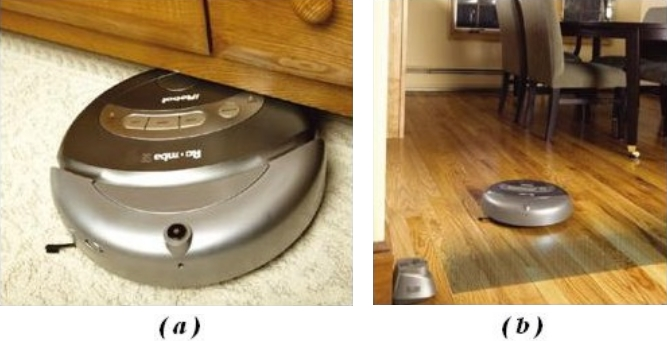
\includegraphics[width=8cm]{figs/roomba}
%  \end{center}
%  \caption{Robot aspirador Roomba de iRobot.}
%  \label{fig:roomba}
%\end{figure}\
%
%Ni tampoco olvides de poner las URLs como notas al pie. Por ejemplo, si hablo de la Robocup\footnote{\url{http://www.robocup.org}}.
%
%\subsection{Números}
%\label{sec:subseccion}
%
%En lugar de tener secciones interminables, como la Sección \ref{sec:miseccion}, divídelas en subsecciones.
%
%Para hablar de números, mételos en el entorno \textit{math} de \LaTeX, por ejemplo, $1.5Kg$. También puedes usar el símbolo del Euro como aquí: 1.500\euro.
%
%\subsection{Listas}
%
%Cuando describas una colección, usa \texttt{itemize} para ítems o \texttt{enumerate} para enumerados. Por ejemplo:
%
%\begin{itemize}
% \item \textit{Entorno de simulación.} Hemos usado dos entornos de simulación: uno en 3D y otro en 2D.
% \item \textit{Entornos reales.} Dentro del campus, hemos realizado experimentos en Biblioteca y en el edificio de Gestión.
%\end{itemize}\
%
%\begin{enumerate}
% \item Primer elemento de la colección.
% \item Segundo elemento de la colección.
%\end{enumerate}\
%
%\paragraph{Referencias bibliográficas}
%\label{sec:referencias}
%
%Cita, sobre todo en este capítulo, referencias bibliográficas que respalden tu argumento. Para citarlas basta con poner la instrucción \verb|\cite| con el identificador de la cita. Por ejemplo: libros como \cite{vega12e}, artículos como \cite{vega19b}, URLs como \cite{vega19a}, tesis como \cite{vega18b}, congresos como \cite{vega18a}, u otros trabajos fin de grado como \cite{vega08b}.
%
%Las referencias, con todo su contenido, están recogidas en el fichero \texttt{bibliografia.bib}. El contenido de estas referencias está en formato \texttt{BibTex}. Este formato se puede obtener en muchas ocasiones directamente, desde plataformas como \texttt{Google Scholar} u otros repositorios de recursos científicos.
%
%Existen numerosos estilos para reflejar una referencia bibliográfica. El estilo establecido por defecto en este documento es APA, que es uno de los estilos más comunes, pero lo puedes modificar en el archivo \texttt{memoria.tex}; concretamente, cambiando el campo \verb|apalike| a otro en la instrucción \verb|\bibliographystyle{apalike}|. 
%
%\
%
%\
%
%\
%
%Y, para terminar este capítulo, resume brevemente qué vas a contar en los siguientes.
